\section{BNF}


La notation BNF (Backus Naur Form)  a été
introduite par John Backus et Peter Naur
 pour décrire le langage de programmation Algol 60.

Plus précisement, elle a été (en grande partie) inventée par
Backus pour décrire Algol 58 dans un rapport de recherche.
Et Peter Naur (qui travaillait sur le même langage) 
s'est alors aperçu qu'il voyait autrement
la syntaxe d'Algol 58.

Ils ont donc décidé, pour le travail
sur Algol, 
de distribuer des descriptions écrites de la 
syntaxe pour que tout le monde parle de la même chose
lors des réunions du groupe de travail. 

{\scriptsize
Source : \url{http://cui.unige.ch/db-research/Enseignement/analyseinfo/AboutBNF.html}}

\subsection{BNF de base}

La notation de base (historique) de la BNF est simple 
\begin{itemize}
 \item la chaîne ``\texttt{::=}'' signifie ``\emph{est défini par}'',
\item la barre \verb+|+ sépare des alternatives,
\item les chevrons ``\verb/<...>/'' entourent des noms de catégories,
\item les éléments terminaux sont représentés tels quels,
\end{itemize}
et se traduit directement en grammaire formelle.

\textbf{Exemple}
\begin{lstlisting}[frame=single]
<program> ::=  program
                   <déclarations>
               begin
                   <instructions>
               end ;

<instruction> ::=   <affectation>
                  | <instruction_tant_que>
                  | <instruction_si_alors_sinon>
                  | ...
\end{lstlisting}


Dans des textes plus modernes, on peut avoir d'autres conventions :
terminaux en gras ou en police ``machine à écrire'', non-terminaux
 en italique, etc.

\begin{center}
\emph{program} ::=  \textbf{program} \emph{declarations}
\textbf{begin} \emph{declarations} \textbf{end}
\end{center}

\subsection{Extensions}

Quelques extensions s'avèrent pratiques, elles sont notées
par des \emph{méta-caractères} :
\begin{itemize}
\item des \textbf{crochets} pour entourer les éléments optionnels
\begin{tabbing}
\hspace{3cm} \= \hspace{1cm}  \= \hspace{1cm} \\
\emph{instruction\_si\_alors\_sinon} ::= \\
  \> \textbf{if} \emph{condition} \\
  \> \> \textbf{then} \emph{instruction} \\
  \> \> [ \textbf{else} \emph{instruction} ]  \\
\end{tabbing}

\item des \textbf{accolades} pour les éléments répétés (zero ou plusieurs fois)
\begin{tabbing}
\hspace{3cm} \= \hspace{1cm}  \= \hspace{1cm} \\
\emph{liste\_d'expressions} ::= \\
  \> \textbf{( ) } \\
  \> | \textbf{(} \emph{expression} \{ \textbf{,} \emph{expression} \} \textbf{)}
\end{tabbing}
\item on peut aussi entourer les terminaux 
de guillemets.
\end{itemize}

\paragraph{Exercice :} comment définir les listes d'expressions en BNF de base, 
sans  ces méta-caractères ?

\paragraph*{Un exemple} plus complet, la syntaxe de la BNF ... en BNF

\begin{lstlisting}[frame=single]
syntax     ::=  { rule }
rule       ::=  identifier  "::="  expression
expression ::=  term { "|" term }
term       ::=  factor { factor }
factor     ::=  identifier |
                quoted_symbol |
                "("  expression  ")" |
                "["  expression  "]" |
                "{"  expression  "}"
identifier ::=  letter { letter | digit }
quoted_symbol ::= """ { any_character } """
\end{lstlisting}

\subsection{Exercices}
\paragraph{Le langage PL/0} de N. Wirth est décrit par une grammaire
de type E-BNF (extended BNF). Ecrivez quelques programmes dans ce langage.
{\small
\begin{lstlisting}[frame=single,numbers=left]
 program = block "." .
 
 block =
     ["const" ident "=" number {"," ident "=" number} ";"]
     ["var" ident {"," ident} ";"]
     {"procedure" ident ";" block ";"} statement .
 
 statement =
     ident ":=" expression
     | "call" ident
     | "begin" statement ";" {statement ";"} "end"
     | "if" condition "then" statement
     | "while" condition "do" statement .
 
 condition =
     "odd" expression
     | expression ("="|"#"|"<"|"<="|">"|">=") expression .
 
 expression = ["+"|"-"] term {("+"|"-") term} .
 
 term = factor {("*"|"/") factor} .

 factor =
     ident
     | number
     | "(" expression ")" .

\end{lstlisting}

\paragraph{Exercice.} Voici des exemples de déclarations de type en 
langage Pascal. Fournissez une grammaire qui couvre au moins
les exemples :

\begin{verbatim}
type chaine = array [1 .. 30] of char;
type date = record 
               jour : 1..31;
               mois : 1..12;
               annee : integer
            end;
type personne = record
                  nom, prenom : chaine;
                  naissance   : date
                end;
\end{verbatim}
Notez qu'en Pascal le point-virgule est un séparateur, alors qu'en C c'est un 
terminateur. Il est donc facultatif après le dernier élément d'un \emph{record}.

                   
\paragraph{Exercice. } Voici un programme écrit dans un langage jouet
\begin{verbatim}
function fac(n)
  local r = 1, i
  for i = 1 to n do
    let r = r * i
  endfor
  return r
endfunction

let encore = 1
while encore == 1 do
  print "valeur de n ? "
  read n
  if n < 0 
  then 
     print "n est négatif"
     let encore = 0
  else 
     let r = fac(n)
     print "factorielle ", n, " = ", r
  endif
endwhile  
\end{verbatim}

Fournir une description du langage en BNF étendue.


\section{Diagrammes syntaxiques}


Les diagrammes syntaxiques expriment essentiellement la même chose que la BNF
mais sous une forme plus facile à appréhender

Exemple : les expressions arithmétiques.

{\scriptsize

\url{http://commons.wikimedia.org/wiki/File:Diagrammes_Syntaxiques.png}
}

\begin{center}
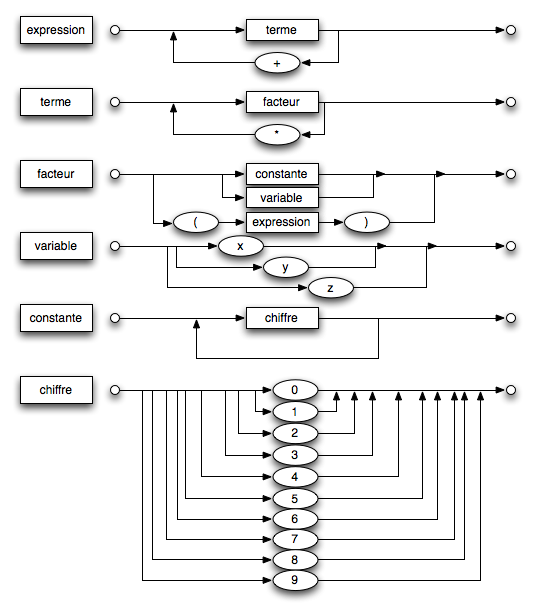
\includegraphics[width=\linewidth]{../images/Diagrammes_Syntaxiques}
\end{center}

Les diagrammes syntaxiques peuvent être vus comme des programmes
(visuels) qui décrivent l'analyse d'une chaine de caractères, en
termes d'appels de sous-programmes : pour reconnaître une expression,
il faut d'abord reconnaitre un terme. Pour reconnaitre un terme
il faut d'abord reconnaitre un facteur, etc.

C'est la base de la technique d'analyse récursive descendante,
technique élégante qui a été appliquée dans nombre de compilateurs
``écrits à la main''\footnote{En effet, une autre option est d'utiliser un programme qui fabriquera un
automate à pile à partir d'une grammaire du langage à reconnaitre.}

\subsection{Déterministe ou pas ?}

A certains endroits du diagramme il y a des fourches, ce qui laisse craindre
un non-déterminisme. Par exemple, dans
\emph{constante}, si on rencontre un second \emph{chiffre}, doit-on 
boucler, ou sortir ?

De préférence, on voudra un analyseur déterministe, il faut donc
étudier la grammaire sous-jacente pour montrer qu'on n'a en fait
jamais le choix.

\paragraph{Méthode. } on regarde en particulier 
\begin{itemize}
\item l'ensemble $First(N)$ 
des terminaux qui peuvent apparaître en première position d'un
non-terminal $N$.
\item l'ensemble $Follow(N)$ 
des terminaux qui peuvent apparaître après un
non-terminal $N$.
\end{itemize}

\paragraph{Pour \emph{First},} on a évidemment 
\begin{itemize}
\item $First(Chiffre) = \{ 0 .. 9 \} $ 
\item et 
$First(Variable) = \{ x, y, z \} $.
\item et donc $First(Constante) = First(Chiffre) = \{ 0 .. 9 \} $
\end{itemize}
Par conséquent, les trois branches de la fourche d'entrée de
\emph{facteur} correspondent à des cas disjoints (le troisième est une
parenthèse ouvrante), le choix peut même se faire en regardant
seulement un seul caractère de la chaîne d'entrée.

\paragraph{Pour \emph{Follow.}}
Les flèches de boucle posent la question de savoir si un ``+''
peut suivre une \emph{expression}, une étoile un terme, un chiffre une
constante. Donc de savoir dans quels contextes on peut rencontrer ces
non-terminaux, \emph{dans une chaîne valide}.

On suppose donc que le but est d'analyser une expression isolée, donc
qu'on a une règle liant l'axiome$S$, les expressions et $\$$ une
marque de fin.
$$ S \rightarrow  \mbox{expression} \ \$ $$
De cette règle en déduit immédiatement que
$$\$ \in Follow(expression) $$

Du troisième diagramme, on tire aussi qu'une parenthèse 
fermante (notons-l $f$)
peut suivre une expression : $f \in Follow(expression) $.

Un certain nombre d'inclusions se déduisent également :
si un symbole peut suivre une expression, alors
il peut aussi suivre un terme (diag. 1). Un plus peut aussi suivre un terme.


\subsection{Un systeme d'inequations}

\paragraph{Le tableau ci-dessous} résume nos trouvailles

\begin{center}
\begin{tabular}{|l|rcl|}
\hline
origine &  & \\
\hline
axiome & $\$ $& $\in $&$ Follow(expression)$ \\
diag. 1  & $Follow(expression)$ & $\subseteq $&$  Follow(terme)$ \\
diag. 1  & $"+"$ & $\in  $&$ Follow(terme)$ \\
\hline
diag. 2  & $Follow(terme)$ & $\subseteq $&$  Follow(facteur)$ \\
diag. 2  & $"*"$ & $\in $&$  Follow(facteur)$ \\
\hline
diag. 3  & $Follow(facteur) $&$ \subseteq $&$  Follow(constante) $\\
diag. 3  & $Follow(facteur) $&$ \in $&$  Follow(variable) $\\
diag. 3  & $f$ & $\in $&$  Follow(expression)$ \\
\hline
diag. 4  & $First(chiffre) $ & $ \subseteq $&$  Follow(chiffre) $\\
diag. 4  & $First(constante) $&$ \subseteq $&$  Follow(chiffre) $\\
\hline
\end{tabular}
\end{center}

C'est un système d'inéquations sur des ensembles ; nous en cherchons les 
plus petites solutions.

Pas de panique, la résolution n'est pas compliquée, elle se fait par
un algorithmes itératif :
\begin{itemize}
\item on part d'ensembles vides $E, T, F, Co, V, Ch$ qui représentent
les différents ``follow''.
\item on exécute une boucle qui interprète chaque inéquation comme
une affectation 
\begin{itemize}
\item la première ajoute $\$$ à $E$
\item la seconde ajoute le contenu de $E$ à $T$,
\item etc. 
\end{itemize}
\item il n'y a qu'un nombre fini de symboles, et on ne fait qu'ajouter des éléments, au bout d'un certain
nombre de tours la situation va se stabiliser : on s'arrête.
\end{itemize}


\subsection{Use the computer, Luke}

L'ordinateur qui est votre ami va calculer la solution
en moins de deux, si on écrit un programme Python comme celui-ci
\begin{lstlisting}[language=python, frame=single, numbers=right]
from copy import deepcopy

F = { "e" : { "dollar", "fermante"}, 
      "t" : { "+"}, 
      "f" : { "*" }, 
      "co" : set(), 
      "v" : set(), 
      "ch" : {"chiffre"} }

def m(src, dst):
  F[dst].update(F[src])

n = 0
while True :
  n = n + 1
  old = deepcopy(F)
  m("e", "t")
  m("t", "f")
  m("f", "co")
  m("f", "v")
  m("co", "ch")
  if old == F : break

print ("arret apres %d iterations" % n)
for k in F:
  print (k + " => " + str(F[k]))
\end{lstlisting}

On obtient le résultat
\begin{lstlisting}
arret apres 2 iterations
ch => set(['chiffre', '*', 'dollar', 'fermante', '+'])
co => set(['+', '*', 'dollar', 'fermante'])
f => set(['fermante', '+', '*', 'dollar'])
t => set(['fermante', '+', 'dollar'])
v => set(['+', '*', 'dollar', 'fermante'])
e => set(['dollar', 'fermante'])
\end{lstlisting}

Donc, résumons, les diagrammes syntaxiques sont déterministes parce que
\begin{itemize}
\item après une expression il ne peut pas y avoir un ``+'' (diag. 1)
\item un facteur ne peut pas être suivi par ``*'' (diag. 2)
\item une constante ne peut pas être suivie par un chiffre (diag. 3)
\end{itemize}

\subsection{Compléments}

\begin{itemize}
\item Ici nous avons montré qu'on peut choisir son chemin 
dans le diagramme de l'exemple, en regardant seulement le prochain
caractère de la chaine à analyser.

Certains langages nécessitent de regarder plusieurs caractères. 

\item En C, C++,
c'est même plus compliqué : le nombre d'éléments à lire pour différencier,
par exemple, une affectation d'un appel de fonction n'est pas borné. 
Voyons par exemple 
\begin{verbatim}
 f(....);
 g(....)->a = b; // g fonction qui retourne un pointeur
\end{verbatim}
et l'analyse syntaxique doit donc se baser également sur les types
déclarés.

\item Le calcul de $First$ et $Follow$  est un petit peu plus compliqué
quand les non-terminaux peuvent produire un mot vide. Si on a une règle
$$A \rightarrow B C $$, $First(A)$ contient $First(B)$, mais aussi
$First(C)$ si $B$ peut produire le mot vide. Et aussi $Follow(A)$ si
$B$ et $C$ produisent le vide.

$First(A)$ doit alors être interprété comme ``le premier symbole que
je peux rencontrer si je vais vers un bloc $A$ dans le diagramme''.
\end{itemize}

Tout ceci est fort intéressant et mérite d'être étudié de plus près,
vous en saurez plus si vous continuez en Mastère ou Ecole d'ingénieur
d'informatique.

\section{Descente récursive, un exemple}

Le programme ci-dessous analyse une expression arithmétique, et en fournit
une paraphrase.

Voici le résultat des tests

\lstinputlisting[frame=single,breaklines=true]{../src/lecture-expr.run}

et le source dans les pages qui suivent.

\begin{landscape}

\lstinputlisting[language=c++,frame=single,numbers=left,breaklines=true]{../src/lecture-expr.cxx}

\end{landscape}


